\documentclass[a4paper,fleqn,usenatbib]{mnras}
%\usepackage{newtxtext,newtxmath}
\usepackage[T1]{fontenc}
\usepackage{ae,aecompl}
\usepackage{graphicx}	% Including figure files
\usepackage{amsmath}	% Advanced maths commands
\usepackage{amssymb}	% Extra maths symbols
\usepackage{hyperref}

\def\grs{{GRS\,1739--278\,}}
\def\swiftx{{\em Swift-XRT\,}}
\def\swiftb{{\em Swift-BAT\,}}
\def\xmm{{\em XMM-Newton\,}}
\def\nustar{{\em NuSTAR\,}}
\def\integral{{\em INTEGRAL\,}}
\def\maxi{{\em MAXI\,}}


\def\ferg{erg~cm$^{-2}$~s$^{-1}$}
\def\arcsec{''}
\def\degr{$^\circ$}
\def\arcmin{'}
\def\iaucirc{{IAU~Circ.}}

\title[Study of low-frequency QPO in \grs]{Study of low-frequency quasi-periodic oscillations in \grs during 2014 outburst}

%\author[I. A. Mereminskiy et al.]{
%Ilya A. Mereminskiy,$^{1}$\thanks{E-mail: i.a.mereminskiy@gmail.com}
%Andrey N. Semena,$^{1}$
%Sergey Bykov,$^{1,2}$
%Ekaterina V. Filippova$^{1}$
%\\
% List of institutions
%$^{1}$Space Research Institute, Russian Academy of Sciences, Profsoyuznaya 84/32, 117997 Moscow, Russia\\
%$^{2}$MGTU, Moscow, Russia\\
%}

\author[Authors]{
Authors$^{1}$
\\
% List of institutions
$^{1}$Space Research Institute, Russian Academy of Sciences, Profsoyuznaya 84/32, 117997 Moscow, Russia\\
%$^{2}$MGTU, Moscow, Russia\\
}


\date{Accepted XXX. Received YYY; in original form ZZZ}

\pubyear{2017}

\begin{document}
\label{firstpage}
\pagerange{\pageref{firstpage}--\pageref{lastpage}}
\maketitle

\begin{abstract}
\end{abstract}
We detected low-frequency quasi-periodic oscillations (QPOs) at 0.3..2 Hz in \nustar and \swiftx observations of black hole candidate \grs during its 2014 outburst.

\begin{keywords}
X-rays: individual (\grs)  -- accretion, accretion disks	
\end{keywords}


\section{Introduction}
\label{sec:intro} 
A study of X-ray variability in accreting astrophysical sources provides a broad view on processes that take a place in such systems. This works both on a long timescales - i.e. days and weeks - when one speak about state changes through outbursts of transients sources  \citep[see e.g.][]{2005Ap&SS.300..107H, heil15}, and on short - all the way down to milliseconds - when the subject under consideration are a quasi-periodic oscillations (QPOs). By simultaneous usage of spectral and timing data one can better constrain geometry of accretion flow around compact objects and infer on which processes are responsible for generation of observed spectro-timing features in a self-consistent way.

Some aspects of the spectro-timing evolution of the X-ray transients (usually black-hole candidates, BHC) during outbursts can be explained in the frame of the two-temperature accretion flow model \citep{1975ApJ...199L.153E, 1976ApJ...204..187S, 1995ApJ...452..710N}, in which geometry of system consists of the geometrically thin cold disk and geometrically thick hot flow (corona), which is thought to be responsible for production of strong variability. As example, using frequency-resolved spectroscopy \citet{2001MNRAS.321..759C} shown that variable part of the emission has a hard spectrum, produced by Comptonization of soft photons onto hot electrons in the corona, while stable part of the emission has a spectrum which is consistent with the cold classical $\alpha$-disc spectrum \citep{shakura73}.  \cite{1997MNRAS.292..679L} proposed that observed strong variability (seen as a broad band noise in power spectra) is produced due to the stochastic variations of the angular momentum transport efficiency. In this propagating fluctuation model broad band noise is a product of noise signals from different radii of the accretion flow, each with its own characteristic time-scale \citep[see, e.g.][]{2006MNRAS.367..801A, 2013MNRAS.434.1476I}. Therefore, the shape of the broad band noise is determined by the physical and geometrical properties of the accretion flow, e.g. in particular in these works it was suggested that the broad noise dumping frequency is connected to the inner edge of the accretion flow. 

Another feature, frequently observed in the X-ray binaries power spectra is different types of low and high frequency QPOs, manifesting itself as a narrow Lorentzian components. One of the long-standing questions in X-ray timing is the origin of so called type-C low-frequency QPOs \citep[see][for LFQPO classification]{casella05}, which are often found in X-ray binaries harboring both neutron stars and black-holes \citep{wijnands99} during initial rise and transition to disk dominated state (in low-hard state (LHS) and in hard intermediate state (HIMS)), according to standard scheme \citep{grebenev97, tanaka96, remillard06, belloni10}). This QPOs are widespread and easy to detect and study, since they occur at moderate frequencies of 0.1..10 Hz and prominent, having $rms\approx10\%$. Different author prescribe generation of this QPOs to various processes: Lense-Thirring precession of inner parts of accretion disk \citep{stella98, ingram09}, oscillations of standing shock \citep{molteni96}, accretion rate modulation caused by different phenomena \citep{tagger99,cabanac10} e.t.c. In some models, particularly in relativistic precession models (RPM), observed frequency is strongly dependent on location of inner part of cold accretion disk.  

Recent advances in simulating the reflection \citep{ross05,garcia14}, arising from reproduction of emission from central engine by accretion disk, led to the possibility to study geometry of accretion disk in bright systems. For such a study to be made it is essential to obtain broadband X-ray spectrum with high energy resolution - reflected component manifest itself by a presence of prominent, wide and asymmetric iron $K_{\alpha}$-line at 6.4 keV and Compton-hump at 20-30 keV. Now, adding information from X-ray timing one can, in principle, constrain the location of a component, responsible for the variability - which is though to be corona or jet foundation. This task present a challenge, that can be solved only by a telescope that posses both possibility to measure broadband spectrum with good resolution and have a corresponding timing capabilities. \nustar\, \citep{harrison13_nust}, launched in 2013, is the best available instrument for such studies, although, except for observations in energy band above 12 keV, \xmm (and {\it NICER} in the nearest future) can be used too, producing some great results \citep{ingram16}. 

In this article we report on first detection of this QPOs in HIMS of Galactic black-hole candidate \grs\, and present a detailed study of properties of the X-ray variability, along with spectral evolution.

\section{GRS 1739-278}

\grs is a typical X-ray nova, discovered during outburst in 1996  \citep{paul96} by {\it SIGMA} \citep{paul91} telescope onboard {\it GRANAT} space observatory.
Using {\it ROSAT} observation \cite{greiner96} inferred distance of 6--8.5~kpc, indicating that source may belong to Galactic bulge. Optical and radio emission were detected during the course of outburst \citep{hjellming96,marti97}. \cite{borozdin98} found spectral evolution throughout outburst to be consistent with canonical model - outburst starts from LHC, then soft component, associated with disk emission starts to dominate, heralding transition to high-soft state. Eventually, they observed very high state and detected a  QPO at 5 Hz using {\it RXTE} data \citep{borozdin00}.

After some 18 year slumber \grs\, demonstrated another big outburst, rise of which was detected by \swiftb \citep{krimm14_atel} along with \integral \citep{filippova14}. During this outburst extensive observing campaign by \swiftx\, were carried out, along with single long \nustar\, exposure. We will utilize this data in following chapters. After this outburst source remain active with repetitive mini-outbursts \citep{mereminskiy16,yan17}.



\begin{figure*}
\centerline{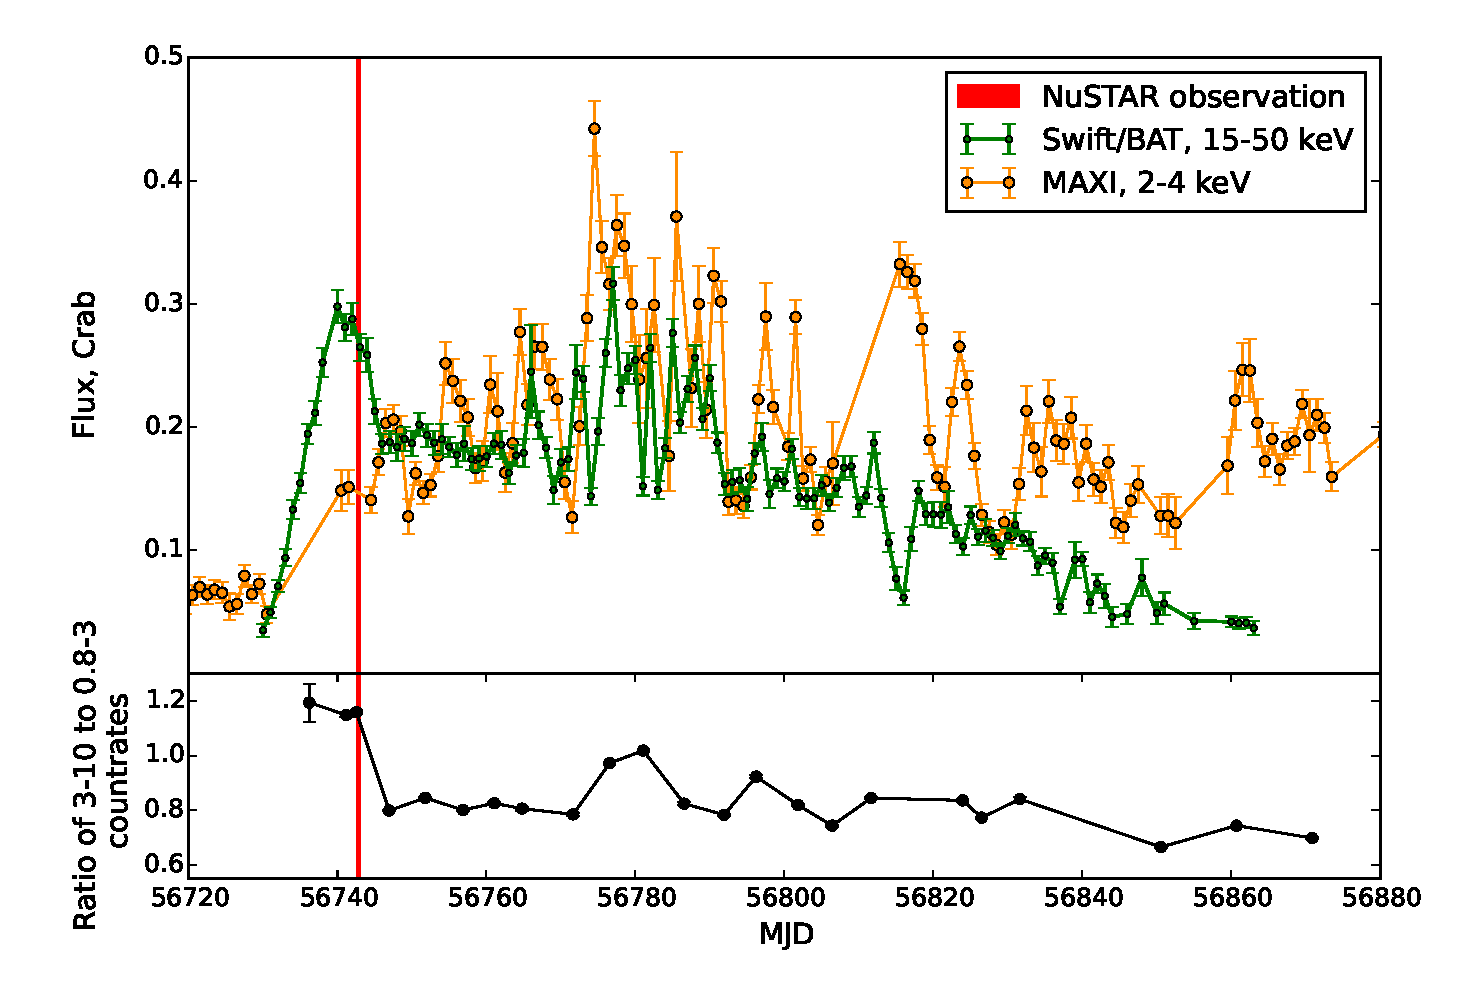
\includegraphics[scale=0.5]{batlc_v06.eps}}
\caption{{\it Upper:} green points denote \swiftb\, lightcurve of second outburst in 15--50 keV range, orange circles correspond to \maxi\, fluxes in 2--4 keV. Red line show time of \nustar\, observation. {\it Lower:} evolution of \swiftx\, spectral hardness during the outburst.} 
\label{fig:batlc}
\end{figure*} 

\section{Observations and data reduction}
\label{sec:datared} 
In order to characterize the overall outburst profile we used data of \swiftb\, {\it transient monitor} \citep{krimm13bat} in hard X-rays (15--50 keV) as well as data from \maxi\, \citep{matsuoka13maxi} (2--4 keV).

We used public observations of \swiftx\, (target ID: 33203) performed regular over the peak and decline of the outburst.  Since the source was bright, all \swiftx\, observations were performed in windowed mode, allowing study of timing properties of the source. We performed standard analysis with {\texttt{xrtpipeline}} and barycentered data prior to lightcurve extraction. During several observations countrate was as high as 280 cts s$^{-1}$, therefore we excluded one or few brightest columns, in order to suppress effects caused by photon pile-up. Photons with energies below 0.8 keV and above 10 keV were also filtered out. 
Long-term lightcurves and spectra were obtained from UK Swift Science Data Centre at the University of Leicester \citep{evans09}.

We also used \nustar\, observation (ObsID: 80002018002) performed at March 26, 2014 (MJD 56742).  {\texttt{nuproducts}} pipeline were utilized to extract photons  from two-arcminute circular region, centered on source and to produce lightcurves and spectra.

\section{Analysis}
\subsection{Outburst}
First detection of the source by \swiftb\, \citep{krimm14_atel} occurred at March 9, 2014 (MJD 56725, we will refer to this date as $\tau_{0}$). Outburst profile in hard X-rays (15--50~keV) featured fast rise with tenfold intensity increase over ten days, nearly flat-top peak ($\tau_{0}$+10..+15) followed by abrupt flux decrease by 30\% over two days. After this, source demonstrated gradual decline interrupted by flaring activity at $\tau_{0}$+30..+65. Another interesting feature is dip, observed in \swiftb\, lightcurve at $\tau_{0} \approx +86$. After the cease of the outburst source remained active with flux about 5--15 mCrab. 

Adding softer data from \maxi\, to the \swiftb\, hard X-ray lightcurve gives us another insight on evolution of the outburst as shown in Fig.\,\ref{fig:batlc} - comparing fluxes in soft and hard bands (for 2--4 keV band we took a 1.67 counts s$^{-1}$ as a reference value for Crab, corresponding value for 15--50 keV band is 0.22 cts cm$^{-2}$ s$^{-1}$) one can see that soft component obviously lags hard emission in the beginning of the outburst but then start to grow and ends up dominating during the flaring period as well as hard dip(s). Lower subplot of Fig.\,\ref{fig:batlc} shows evolution of hardness ratio (3--10~keV/0.8--3~keV) measured by \swiftx. Right after peak of hard X-rays one can see decline of hardness, also indicating appearance of thermal component.

Fortunately, the \nustar\, observation triggered by \cite{miller15_nust} were carried right at the transition between hard and soft states, thus giving us unique possibility to study processes that happens during HIMS. 

\subsection{NuSTAR observation}
\label{sec:nust} 

\nustar\, observed \grs (ObsID: 80002018002) for nearly 30 ks of dead-time corrected exposure right after hard X-ray peak (see Fig.~\ref{fig:batlc}). Earlier, \cite{miller15_nust} shown that the average spectrum of this observation is well described by reflection models such as {\it relxill} \citep{garcia14, dauser14,dauser16} with accretion disk that reaches remarkably close to the black hole innermost stable circular orbit (ISCO), with upper estimate being $r_{in} = 5^{+3}_{-4}\, G M/c^{2}$ \citep{miller15_nust}. Interestingly, no additional thermal component was needed in order to obtain a good fit, probably because of \nustar\, energy band, starting at 3~keV. 

Given the 96.9 minute orbital period of \nustar, observation is divided in 13 intervals separated by Earth occultations, as shown in Fig.\,\ref{fig:nust_lc}. We denoted this intervals with roman numerals, from {\bf I} to {\bf XIII}. From the lightcurve of observation it is clear, that source flux is increasing throughout observation from $\approx$145 counts per second up to $\approx$170 counts per second. 
The spectrum also alter, with hardness (defined as ratio of countrates  $R_{3-10\,keV}/R_{10-78\,keV}$) monotonically growing from 2.5 to 3.5. 

\subsubsection{Continuum evolution}
To get better view on evolution of continuum emission we fitted using \texttt{XSPEC} package \citep{arnaud96} all individual interval spectra with \texttt{xillver} model \citep{garcia13}. This model describes reflection of incident radiation from ionized slab of matter. The spectrum of incident radiation are assumed to be power-law with exponential cutoff. Spectra from two \nustar\, modules of each interval were fitted simultaneously with \texttt{phabs*const*xillver} model. We choose to fix interstellar absorption at $N_{H} = 2.15\times10^{22}$ cm$^{-2}$  as was found by joint \xmm/\nustar\, observation during low luminosity state \citep{fuerst16}. Element abundances were taken from \cite{wilms00} and cross-sections from \cite{verner96}. Relative iron abundance were fixed at
 $A_{Fe} = 1$, ionization parameter at $\xi=3.2$ and inclination at 35 degrees. This parameters are in agreement with measured by \cite{miller15_nust} with different spectral models. Although in  \texttt{xillver} there is no relativistic broadening of Fe-line no significant residuals in 5--8 keV region are seen, mainly because of limited statistics in per interval spectra. Before fitting, spectra were grouped in order to have at least 100 counts per bin, channels above 60 keV were ignored. Resulting fits are of satisfactory quality with mean $\chi^{2}_{red.} \approx 1.05$. 
 
Examination of best-fit parameters shown in Fig.\ref{fig:intspe} confirms that spectrum softens during observation and cut-off energy decreases. Flux is steadily increasing and at the end of observation unabsorbed luminosity in 3--60 keV band reach  $7\times10^{37}$ erg s$^{-1}$ assuming 8 kpc distance. 

\subsubsection{Constrains on movement of the inner parts of accretion disk}
Yet, spectra of single intervals have not enough statistics to constrain change of Fe-line profile and, hence, to determine is the inner boundary of disk is moving during observation. To increase statistics, we split whole observation into three major pieces, with first made by intervals {\bf I-IV}, second by {\bf V-IX} and third by {\bf X-XIII} and extracted 4--78 keV spectra. 
We chose to group them in order to have at least 100 counts per bin and then we fitted them (excluding data between 5--10 keV) with simple \texttt{phabs*cutoffpl} model, using, once again, $N_{H} = 2.15\times10^{22}$ cm$^{-2}$.  

Now, plotting the ratio of this fit to initial spectra (see Fig.~\ref{fig:ratios}) one can see that both strong features - i.e. Fe-line complex at 5--9 keV and Compton hump around 30 keV are seemingly stable. Therefore we can conclude, that there is no drastic change in position of inner disk boundary between parts of observation. Additionally, we estimated equivalent width of Fe-line in this three parts - we approximated 4--78~keV spectra with 10--30~keV range being ignored (to neglect the Compton-hump contribution) with model consisting of absorbed cut-off powerlaw and gaussian. Equivalent width of gaussian component remain constant within error margins, around 0.175 keV, although it is possible that the quality of data is not enough to trace the real change.

\begin{figure*}
\centerline{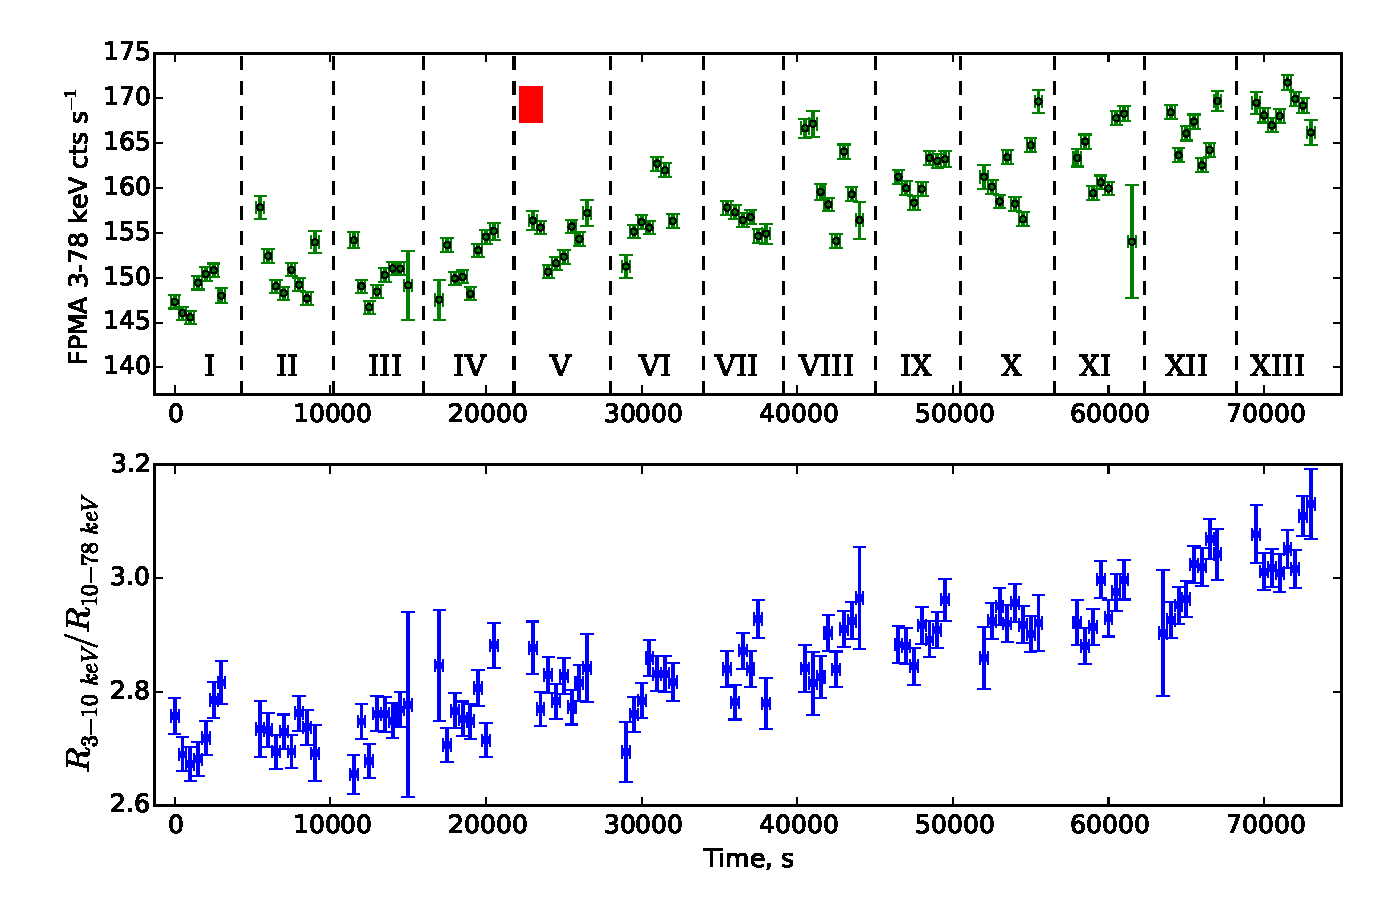
\includegraphics[scale=0.7]{nuAlc_color_v04.eps}}
\caption{Upper panel: countrate of \nustar\,FPMA in 3--78 keV band. We enumerated intervals of uninterrupted observations with roman numerals. Red square shows time of simultaneous \swiftx observation (ObsId: 00033203003, second part). Bottom panel: evolution of hardness during observation} 
\label{fig:nust_lc}
\end{figure*} 
 \begin{figure}
\centerline{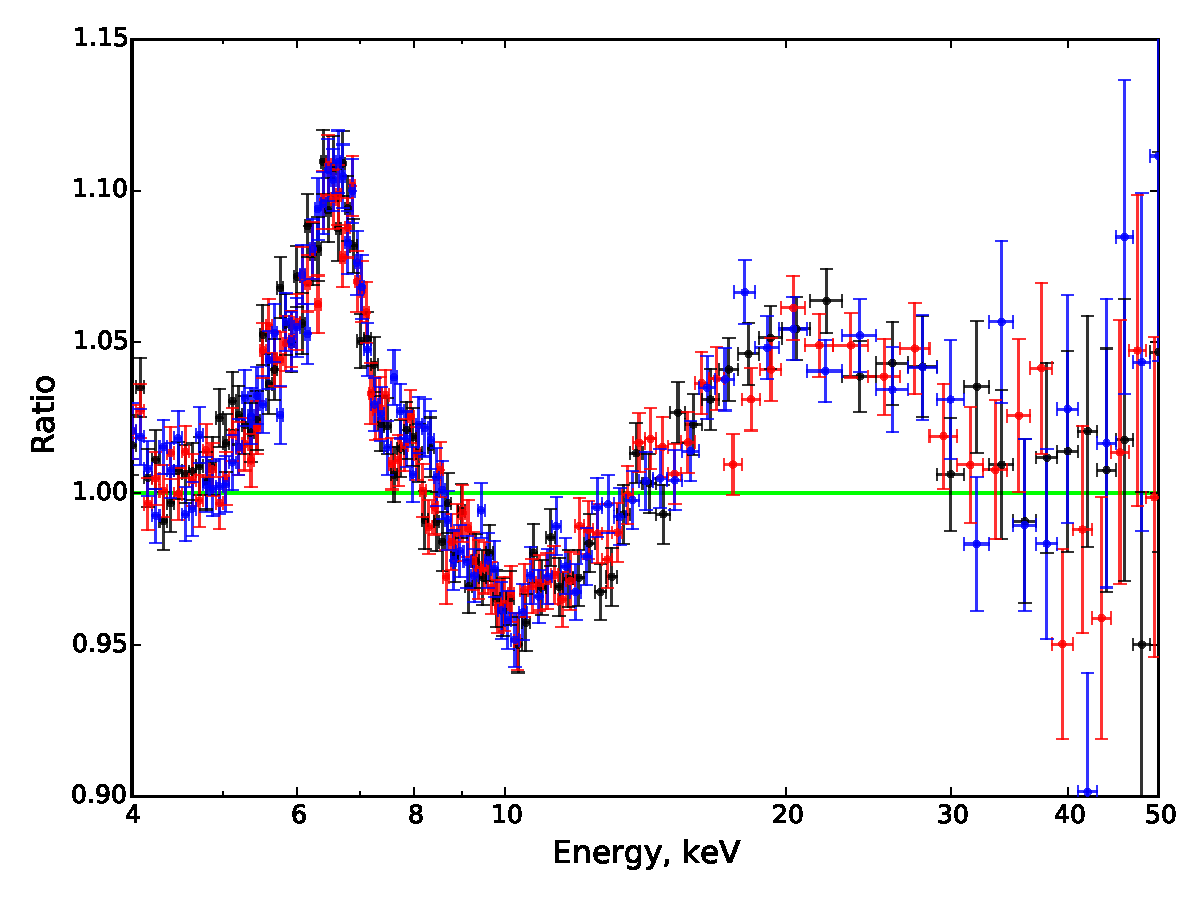
\includegraphics[width=\linewidth]{ratios_v01.pdf}}
\caption{Ratio of \nustar\, FMPA, spectra to \texttt{phabs*cutoffpl} model. In black - data from intervals I-IV, in red from V-IX and in blue from X-XIII.} 
\label{fig:ratios}
\end{figure}  

\begin{figure}
\centerline{\includegraphics[width=\linewidth]{intspe_v02.eps}}
\caption{Parameters of continuum emission in intervals. From upper to lower: \texttt{xillver} powerlaw slope, cutoff energy,  flux in 3--60 keV band $\times$\, erg s$^{-1}$ cm$^{-2}$, $\chi^{2}$ per degree of freedom and Fe-line equivalent width.} 
\label{fig:intspe}
\end{figure}  
            
\subsubsection{Characterization of the average spectrum}            
There is a 1.3 ks part of \swiftx\, snapshot (ObsId: 00033203003) that coincides with \nustar\, observation. Extension of an energy range to 0.8 to 78 keV allow one to search for thermal emission associated with cold inner disk with $kT \sim 0.1...0.4$~keV (such as were found in other BHCs, see \cite[][ e.t.c]{miller06b,miller06a,parker15}).

We extracted \swiftx\, spectrum using only zero-grade events, and grouped it (as well as \nustar\, spectra) to have at least 30 counts per bin and added 3\% systematic error. We used latest available version of {\it relxilllp} package (v1.0.2), the model that describes reflection of emission produced by point source located on the rotation axis above the Kerr black hole from the relativistic accretion disk. Among the parameters of a model several of a particular interest namely $h$ - height of point source above the black hole and $R_{in}$, location of the inner boundary of accretion disk.  This model was selected for several reasons - first, \cite{miller15_nust} found that it match observed data well producing least strigthent constraints on inner radius of the disk. Also, during the 1996 outburst source was detected at radiowaves, possibly indicating jet activity.

Interestingly, instead of surplus thermal component we found a lack of soft emission - usage of $N_{H} = 2.15\times10^{22}$ cm$^{-2}$, measured in source low state \citep{furst16} led to worse fits with systematic negative residuals below few keV. Therefore, we left $N_{H}$ free during the fit. Obtained value of 2.6$\times10^{22}$ cm$^{-2}$ is higher than one measured by \cite{furst16}. This can be possibly accounted to presence of disk outflow, caused by severe X-ray irradiation. 

Other parameter values match well with measurements by \cite{miller15_nust}. 

\begin{table}
\noindent
\centering
\caption{Best-fit parameters of \texttt{phabs*relxilllp} model}
\label{tab:fullfit}
\centering
\begin{tabular}{|c|c|}
\hline\hline
Parameter & Value \\
\hline
$N_{H}$ &   2.65$^{+0.04}_{-0.02}$ \\   
$h$   &  19.2$^{+2.8}_{-2.2}$ \\
$a$    & 0.76$^{+0.21}_{-0.47}$   \\
$incl$ & 24.3$^{+1.7}_{-2.4}$ \\
$R_{in}$  & 1.25000 \\ 
$\Gamma$& 1.40$^{+0.01}_{-0.01}$   \\
$\log{\xi}$ &  3.48$^{+0.04}_{-0.03}$ \\
$A_{Fe}$   &  3.0$^{+0.3}_{-0.2}$  \\        
$E_{cut}$    &       26.2 $^{+0.4}_{-0.3}$    \\
$R_{refl}$  &         0.44$^{+0.03}_{-0.04}$    \\
$N,\,\times10^{-2}$          &      1.54$^{+0.07}_{-0.06}$ \\
$C_{FMPB}$ & 1.018$^{+0.001}_{-0.001}$    \\
$C_{Swift-XRT}$    &   1.04$^{+0.001}_{-0.001}$\\
$\chi^{2}_{red.}$    &   1.1=\\ 
              &= 3366.81/3075 d.o.f\\

\hline
\end{tabular}
\end{table}




\begin{figure}
\centerline{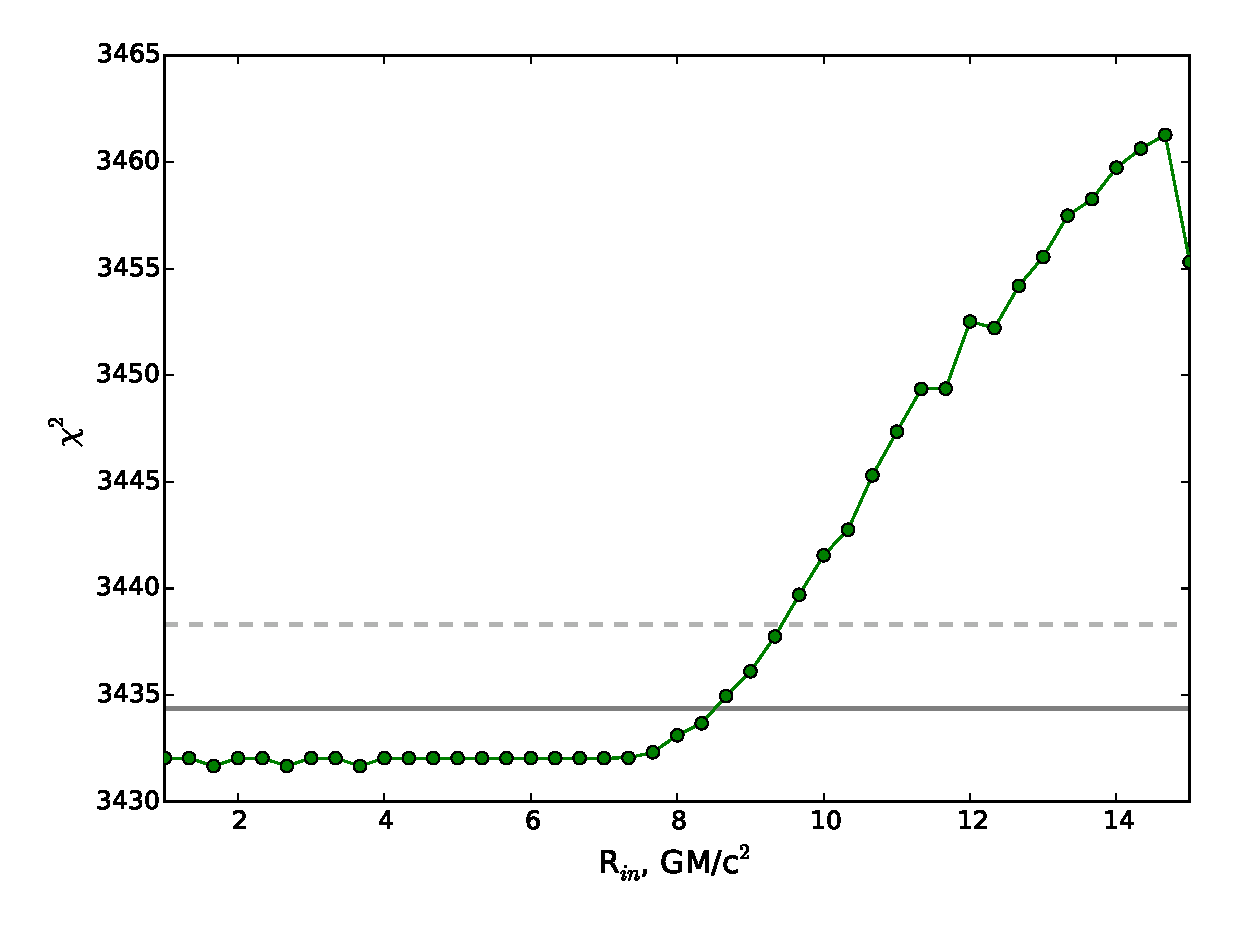
\includegraphics[width=\linewidth]{rinfit_v03.eps}}
\caption{Estimate of inner radius of accretion disk. Gray solid line denote 90\% confidence interval, while dashed line shows 99\% interval.} 
\label{fig:rin}
\end{figure}  


\section{Timing analysis} 
%    Along with the spectral analysis of X-ray transients, timing analysis give a vast of information about the geometry and current state of the accretion flows in such systems. 
%For example, broad band timing variability properties are used in determination of the systems state \cite{2005Ap&SS.300..107H}.
%
%    Variability properties of different types of X-ray binary systems are usually described in terms of the luminosity power spectrum, which is a common technique on determination of amount of power in the particular frequency range.
%    Luminosity variability power spectrum of the transient system typically can be described with a set of broad and thin Lorentzian functions representing correspondingly broad band stochastic noise and QPOs \citep[see, e.g.][]{1972ApJ...174L..35T, 1990A&A...227L..33B}.
%    The overall variability and the shape of the power spectrum changes dramatically with the spectral states of the transients and, in some cases, manifest state transitions even if they are not evident from the energy spectrum.
%
%    Some aspects of the evolution of the X-ray binaries system power spectrum with their state can be explained in the frame of the two-temperature accretion flow model, where it consists of the geometrically thin cold disk and geometrically thick hot flow (corona), particularly it is widely accepted that the high amplitude variability is associated with the geometrically thick flow, while the geometrically thin disk is generally stable \citep{2001MNRAS.321..759C}. 
%It should be noted that this model of the variability generation are directly connected with the models, explaining energy spectra of black hole binaries \citep[see, e.g.,][]{1975ApJ...199L.153E, 1976ApJ...204..187S, 1995ApJ...452..710N}, \citet{2001MNRAS.321..759C} has shown with the frequency resolved spectroscopy that variable part of the emission has a hard spectrum, which is thought to be produced in the corona, while stable part of the emission has a spectrum which is consistent with the cold classical $\alpha$-disc spectrum \citep{ss73}.
%
%    It is generally accepted that the broadband noise observed in the power spectrum of binary systems is produced due to the stochastic variations of the angular momentum transport efficiency \citep{1997MNRAS.292..679L}. 
%    In this propagating fluctuation model broad band noise is a product of noisy signals from different radii of the accretion flow, each with its own characteristic time-scale \citep[see, e.g.][]{2006MNRAS.367..801A, 2013MNRAS.434.1476I}.
%    It follows, that the shape of the broad band noise is determined with the physical and geometrical properties of the accretion flow, e.g. in particular in these works it was suggested that the broad noise dumping frequency is connected to the accretion flow inner edge.
%
%    Another feature, frequently observed in the X-ray binaries power spectra is different types of low and high frequency QPOs manifesting itself as an excessive power in the thing frequency bands. 
%    There is at least five types of these QPOs were observed on the frequencies above 0.1~Hz in the stellar mass binary systems \citep[for classification see][]{2005Ap&SS.300..107H}.
%
%Several models were proposed to explain high and low frequency QPO features in power spectra \citep[][]{1997ApJ...489..865E, 1998ApJ...506..281B, 1998ApJ...492L..59S, 1999A&A...349.1003T, 1999ApJ...518L..95T, 2001A&A...374L..19A, 2009MNRAS.397L.101I, 2011MNRAS.415.2323I}. 
%Changes, observed with the evolution of the spectral states between different types QPOs and broad band noise, e.g. correlation between QPOs centroid frequencies and broad noise dumping frequency \citep{1999ApJ...514..939W, 2014MNRAS.437.2554M} speak in favor of the origin of the QPOs in the inner edge of the accretion flow.
%
%While these models, describing broad band noise and QPOs in the variability power spectrum, usually do not confront observed energy spectra, it was found that some additional demands on time properties must be met.
%\citet{1997ApJ...474L..43V} used coherence spectrum in order to additionally constrain time properties of the accretion flow. 
%They found a time lag between hard and soft emission of the soft and hard emission, which have a complex behaviour with the frequency, which they used to constrain geometrical size of the accretion flow \citep{1999ApJ...517..355N}. 
%Observed time lags also were used to discriminate some spectral models \citep[see, e.g.,][]{2001MNRAS.327..799K}.

 Variability properties of different types of X-ray binary systems are usually described in terms of the power spectrum, which is a common technique for determination of amount of power in the particular frequency range. Power spectrum of the BHC systems in LHS typically can be described as a combination of band-limited noise and one or few narrow Lorentzian functions, representing correspondingly broad band stochastic noise and QPOs \citep[see, e.g.][e.t.c]{1972ApJ...174L..35T, 1990A&A...227L..33B, homan05}. Properties of this components and correlations between them, in principle, may be used to discriminate between different models, proposed for generation of X-ray emission in BHC. 
 
 Although power spectra analysis is by far the most popular, more sophisticated methods, such as coherence function or phase-lag were successfully used to infer physical properties of accretion flows. Using a measured time-lag between the soft and hard emission, which have a complex behavior with the frequency, \cite{1999ApJ...517..355N}  constrained geometrical size of the accretion flow. 

%\citet{1997ApJ...474L..43V} used coherence spectrum in order to additionally constrain time properties of the accretion flow. 
%They found a time lag between hard and soft emission of the soft and hard emission, which have a complex behavior with the frequency, which they used to constrain geometrical size of the accretion flow \citep{1999ApJ...517..355N}. 
%Observed time lags also were used to discriminate some spectral models \citep[see, e.g.,][]{2001MNRAS.327..799K}.

In the following section we present analysis of the timing properties and their evolution during the 2014 outburst of \grs.

\subsection{Power spectrum}
    {\it NuSTAR} observation of the \grs\ 2014 outburst are split on 13 continuous parts separated with $\sim0.7$~hr intervals when the source was occulted by Earth. 
    The continuous observations have duration from $\sim2440$ to $\sim3390$~sec see Table~\ref{}.
    Since {\it NuSTAR} detectors operate in the photons counting mode, data can be reduced to the light-curve with time resolution up to 2$\mu$s.
    For our analysis we extracted light-curves with 0.01~s temporal resolution, therefore we obtained power spectra in the $sim3\times10^{-3}$--$50$~Hz range.
    This is a frequency range which usually contains low frequency quasi periodic oscillations QPOs and broad band noise component \citep{1999ApJ...514..939W}.
    We didn't try to found high frequency QPOs, since the typical HF QPO (centroid frequency 100-400~Hz, amplitude $\approx10$\% and quality $Q\approx0.1$--$0.5$) is indiscernible over the Poisson noise with the obtained count-rate.

    The power spectrum of each of the separate observations has a form of a white noise plateau ($P(f)\propto const$) on the low frequencies, transforming on the frequency $\approx0.1$~Hz in to the power law with the slope $\rho\approx-1.6$--$-2.0$. Also a prominent QPO on the frequencies 0.3--0.7~Hz and its second overtone is presented. Typical power spectrum of single interval is shown in Fig.~\ref{fig:qpo}.
    Poisson noise dominates intrinsic source variability on the frequencies over $\approx2$~Hz, preventing analysis of any high-frequency features. %, nevertheless we inspected power spectrum in the range from 100 to 500~Hz and didn't find any signs of high frequency QPOs.
    There is also signs that the Power spectrum on the frequencies below $\approx0.003$~Hz has a form of growing power law $P(f)\propto f^{\alpha}$, $\alpha > 0$.

    From the shape of the energy and Fourier spectrum we concluded that the system is in the hard intermediate state and observed low frequency QPO (LF QPO) is of type C. 

    In order to assess properties of the variability power spectra we approximate each obtained power spectra with the following analytical function:
\begin{equation}
        \begin{split}
        P(f) = n (1 + (f/f_{\rm lb})^4)^{\alpha} + \\
        \frac{s_1}{(f - f_{qpo})^2 + (f_{\rm qpo} Q_{\rm m})^2} +\\
        \frac{s_2}{(f - 2f_{qpo})^2 + (2f_{\rm qpo} Q_{\rm m})^2} + \\
        + poiss
\end{split}
        \label{eq:complex_fit}
\end{equation}


In this function first component represents plateau with the break, second two components describe QPO main harmonics and its overtone, last component represents constant Poisson noise.

Due to the complex dead-time behaviour over the energy, it's impact on to the power spectrum can not be well described. 
This method is based on the following assumption: since photons arrival times are independent for the two detectors, phases of the Fourier function of two light-curves are also random and independent.
It follows that this cross-product is a complex value with random uniformly distributed phase and the mean of it's real part is zero.
Following \cite{2015ApJ...800..109B} we calling obtained function cross-spectrum or cospectrum. 

While cross-spectrum technique works perfectly for the power spectrum assessment, we still using classical Fourier power spectrum for the analysis in this work due to the following reason.
Each value of the cross-spectrum belongs to the distribution with a complex probability density function (PDF), which,  for the random independent signals in two detectors, can be described with the special Bessel function of second kind and has a different PDF for a coherent signals. 
Since this distribution has finite standard deviation, according to the central limit theorem, distribution of the sum of the values tends toward a normal distribution.
To track the source variability evolution we fitting relatively short observations with duration of 2--3~ks, and therefore can not split them more than to few dozens parts in order to have an eye on the power spectrum break feature on the 0.1~Hz frequency. 
We found that usual root mean square technique, used to fit normally distributed values, works not stable in that case, probably because the PDF is not yet close enough to the normal distribution. 

To simplify our analysis we inspect power spectrum only on frequencies above 10~Hz, allowing Poisson noise to has arbitrary power but assuming that it's power spectrum component is still flat ($P(f) = const$).

\begin{figure*}
        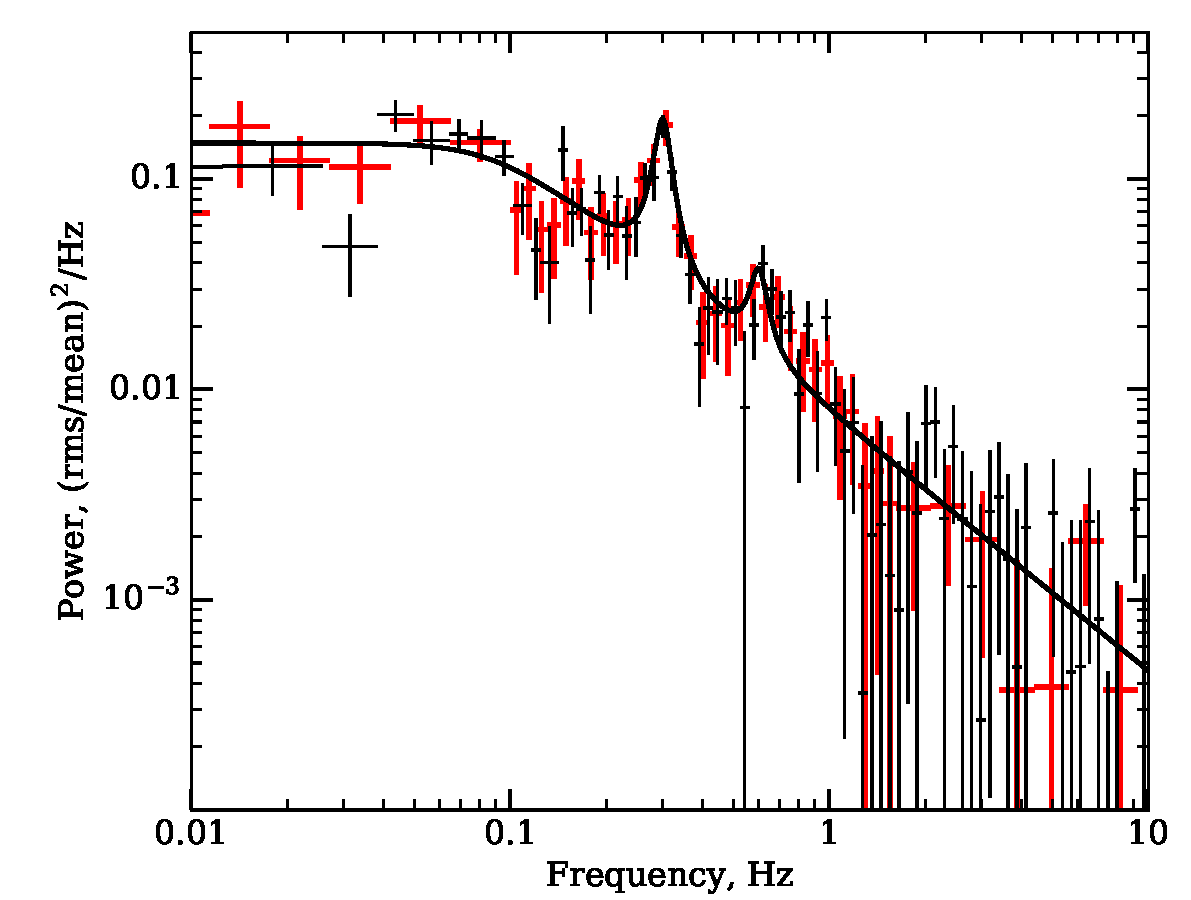
\includegraphics[trim=0 0 0 0.65cm, clip, width=\columnwidth]{spectrum_model_and_cospectrum0.pdf}
        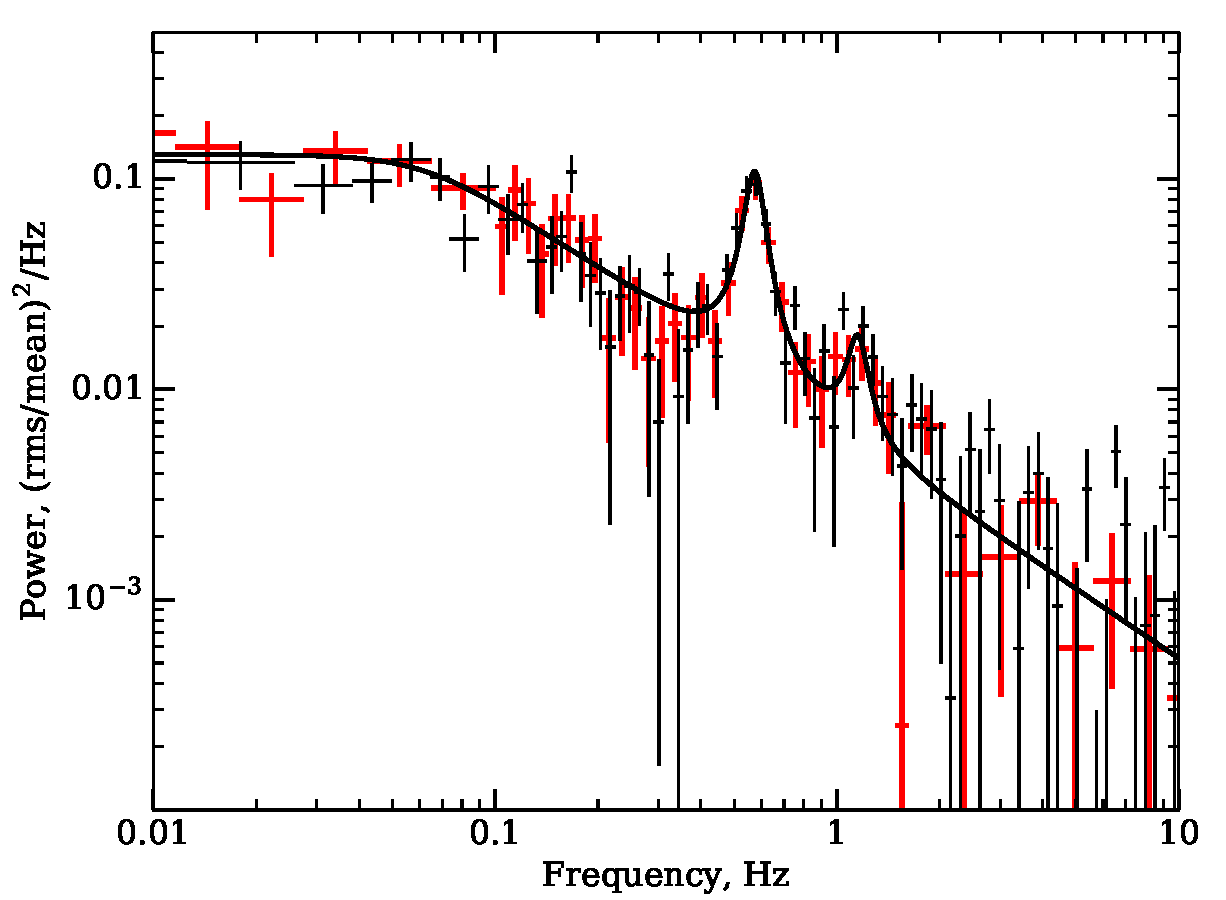
\includegraphics[width=\columnwidth, height = 0.83\columnwidth]{spectrum_model_and_cospectrum10.pdf}
        \caption{On the left panel power spectrum and cospectrum obtained in the soft band at the beginning of {\it NuSTAR} observation. 
        On the right column same spectra obtained at the end of the observation.
        Red crosses correspond to the power spectrum with Poisson noise component subtracted, and black crosses correspond to cospectrum.
        Black line represents best model for the power spectrum without Poisson noise component.}
        \label{fig:qpo}
\end{figure*}


We found that the QPO frequency and amplitude had clearly evolved with time see Table~\ref{tab:ps} and Figure~\ref{fig:qpo}.
The QPO frequency correlates with the {\it NuSTAR} flux and photon index, similar to many other black hole and neutron star binary systems \citep[see, e.g.,][]{2003A&A...397..729V,2003A&A...407.1039P}.
On the other hand we see, that the QPO amplitude was stable during the first half of the observation, and started to grow in the second part.

\begin{table*}
\noindent
\centering
\caption{Evolution of the Fourier and energy spectrum properties through the {\it NuSTAR} observation in the 3--5~keV energy band.}
\label{tab:timing}
\centering
\begin{tabular}{|c|c|c|c|c|c|c|c|c|c|c|}
\hline\hline
Interval & T$_{start}$, & Expo,  & f$_{\rm br}$, & f$_{\rm QPO}$, & Q$_{\rm m}$, & A$_{\rm m}$, & A$_{\rm o}$,& rms, \% & $\Gamma$ & E$_{\rm cut}$, \\
            &  MJD &  s & $\times10^{-2}$, Hz &  Hz & $\times10^{-2}$ & (rms/mean) \% &  (rms/mean) \%   &  & &  keV \\
\hline
I &  	56742.68 & 3386 & $9.0_{-2.5}^{+2.5}$ & $0.30\pm0.01$ & $7.2_{-1.8}^{+2.5}$ & $7.4_{-1.2}^{+1.1}$ & $3.9_{-1.3}^{+1.1}$ & $27\pm3$ & 1.46$\pm$0.01 & $29.9\pm0.4$ \\
II & 56742.75 & 3388 & $8.8_{-2.3}^{+2.6}$ & $0.31\pm0.01$ & $8.5_{-2.2}^{+2.6}$ & $7.6\pm1.2$ & $3.3_{-1.2}^{+1.1}$ & $24_{-2}^{+3}$ & 1.46$\pm$0.01 & $30.7\pm0.4$ \\
III &  56742.81 & 3392 & $9.1_{-2.2}^{+3.2}$ & $0.34\pm0.01$ & $8.7_{-2.2}^{+3.3}$ & $7.2\pm1.2$ & $3.9_{-1.2}^{+1.0}$ & $26\pm3$ & 1.46$\pm$0.01 & $29.7\pm0.4$ \\
IV &  56742.88 & 3389 & $8.3_{-2.1}^{+2.5}$ & $0.35\pm0.01$ & $8.6_{-1.9}^{+2.4}$ & $7.3_{-1.2}^{+1.1}$ & $4.2_{-1.2}^{+1.1}$ & $27_{-3}^{+4}$ & 1.47$\pm$0.01 & $29.5_{-0.3}^{+0.4}$ \\
V &  56742.95 & 3389 & $7.2_{-1.9}^{+2.0}$ & $0.39\pm0.01$ & $8.6_{-2.1}^{+2.7}$ & $7.1_{-1.1}^{+1.0}$ & $4.4_{-1.3}^{+1.2}$ & $27_{-3}^{+4}$ & 1.47$\pm$0.01 & $28.6\pm0.3$ \\
VI &  56743.02 & 3136 & $7.2_{-2.0}^{+2.1}$ & $0.41\pm0.01$ & $7.1_{-1.8}^{+2.0}$ & $7.0\pm1.1$ & $4.8_{-1.2}^{+1.1}$ & $27_{-3}^{+4}$ & 1.47$\pm$0.01 & $28.1\pm0.3$ \\
VII & 56743.09 & 2771 & $8.4_{-2.2}^{+2.5}$ & $0.42\pm0.02$ & $13.0_{-3.0}^{+4.0}$ & $7.3_{-1.3}^{+1.2}$ & $4.1_{-1.2}^{+1.4}$ & $25_{-3}^{+4}$ & 1.50$\pm$0.01 & $28.7\pm0.4$ \\
VIII & 56743.15 & 3387 & $6.0_{-1.7}^{+1.8}$ & $0.46\pm0.01$ & $7.2_{-1.9}^{+2.5}$ & $6.6_{-1.0}^{+1.1}$ & $3.8_{-1.3}^{+1.1}$ & $30_{-5}^{+6}$ & 1.51$\pm$0.01 & $29.3\pm0.4$ \\
IX & 56743.22 & 3392 & $13.0_{-3.0}^{+3.0}$ & $0.49\pm0.02$ & $15.0_{-3.0}^{+4.0}$ & $9.8_{-1.1}^{+0.9}$ & $6.6_{-1.2}^{+1.0}$ & $21\pm1$ & 1.50$\pm$0.01 & $28.1\pm0.3$ \\
X & 56743.29  & 3390 & $7.9_{-2.5}^{+2.4}$ & $0.54\pm0.01$ & $7.8_{-1.8}^{+2.1}$ & $7.9_{-1.0}^{+1.1}$ & $5.3_{-1.0}^{+1.2}$ & $26_{-3}^{+5}$ & 1.50$\pm$0.01 & $27.2\pm0.3$ \\
XI & 56743.35 & 3382 & $6.3_{-1.9}^{+2.3}$ & $0.57\pm0.01$ & $7.8_{-1.7}^{+2.0}$ & $8.3\pm1.0$ & $4.1_{-1.4}^{+1.1}$ & $26_{-3}^{+5}$ & 1.53$\pm$0.01 & $28.7\pm0.3$ \\
XII & 56743.42 & 3386 & $7.1_{-2.2}^{+2.4}$ & $0.63\pm0.01$ & $8.8_{-1.7}^{+2.7}$ & $8.9_{-1.1}^{+1.0}$ & $5.1_{-1.3}^{+1.2}$ & $26_{-3}^{+6}$ & 1.53$\pm$0.01 & $27.5\pm0.3$ \\
XIII &  56743.49 & 3391 & $6.8_{-2.1}^{+2.2}$ & $0.67\pm0.01$ & $6.5_{-1.4}^{+2.0}$ & $8.8_{-0.9}^{+1.0}$ & $4.4_{-1.2}^{+1.1}$ & $27_{-4}^{+6}$ & 1.53$\pm$0.01 & $26.2\pm0.3$ \\
\hline
\end{tabular}
\end{table*}

Some models suggest, that the type-C QPO arising due to the Lense-Thirring precession of the accretion flow inner parts \citep{1998ApJ...492L..59S, 2006ApJ...642..420S, 2009MNRAS.397L.101I}, in such models growth of the QPO frequency corresponds to the shrinking of the disk inner radius.
However, sophisticated spectral models applied to the observed {\it NuSTAR} spectrum suggest that the accretion disk inner radius is $R_{\rm in}= 5_{-3}^{+3}R_{\rm g}$.
This estimation is primarily based on the profile of the relativistically widened neutral Iron fluorescent line, see section~\ref{sec:spec} and also \citep{miller15_nust}.

We found that the QPO amplitude is smaller in the soft band, while amplitude of it's harmonic is bigger, the ratio of the power in the QPO and it's harmonic is $0.2\pm0.1$ in 10--78~keV band and $0.4\pm0.1$ in 3-5 energy band.
It follows that the QPO profile, if it's presented \citep[see, e.g.][]{2015MNRAS.446.3516I}, differs in the hard and soft X-ray band.
Following \citep{2015MNRAS.446.3516I} we tried to extract  QPO profile segregating the coherent part between the QPO and it's harmonic, however no significant coherence was presented above the noise level, one can conclude that the QPO profile was not stable along the observation. 

In some observation segments QPO subharmonics, centered approximately at the 1/2 of the QPO centroid frequency, is clearly observed in the cross-spectra (see examples on Figure~\ref{fig:subharmonic}, red crosses) (namely I, II, IV, V, VI sets).
In order to observe QPO profile with better significance we summarized several cospectra, frequency of each cospectrum was scaled in such a way to conserve QPO centroid at 0.3~Hz.
Obtained ``tracked'' cospectrum is presented on Figure~\ref{fig:cospec_tracked}.
The subharmonics seems to roam around the 1/2 QPO frequency, therefore we were not able to obtain it with a large significance on the tracked spectrum.


\begin{figure}
        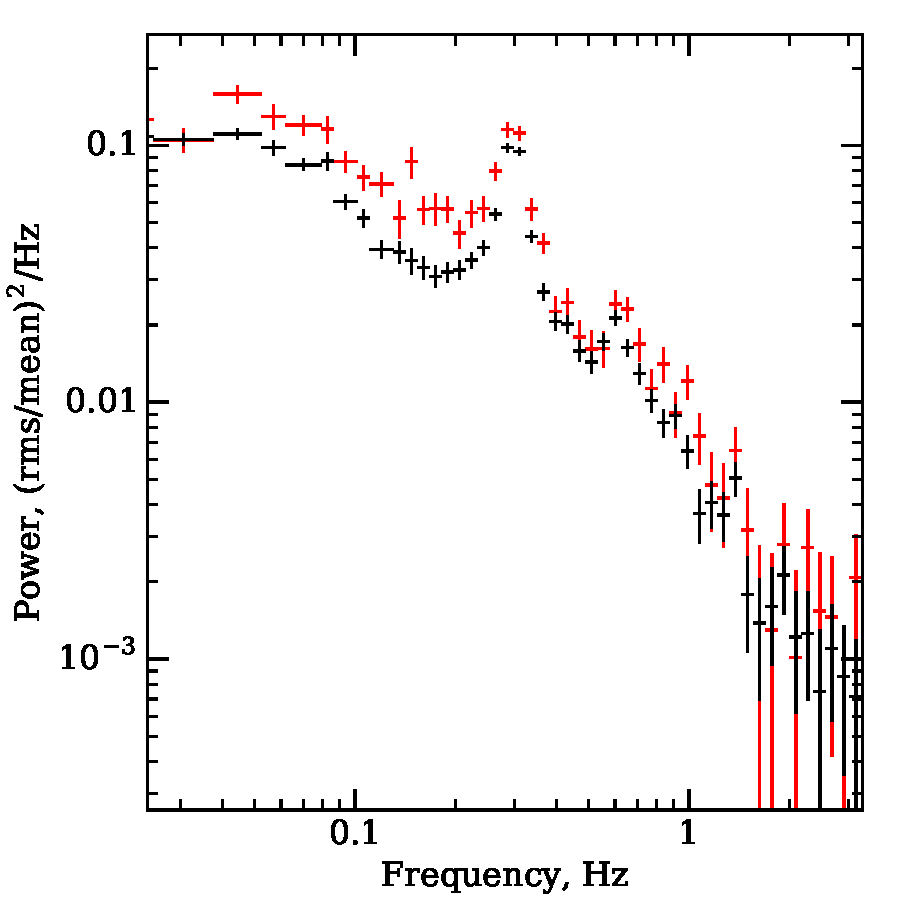
\includegraphics[width=\columnwidth]{folded_cospectr2.pdf}
        \caption{Cross-spectrum of the observations, obtained by scaling frequency to conserve QPO position.
        Black crosses obtained from the all data sets, while red crosses are from sets I, II, IV, and V, in which QPO subharmonics was most prominent.}
        \label{fig:cospec_tracked}
\end{figure}

It should be noted that the changes in the QPO centroid position during the interval may contribute to the observed quality factor $Q$.
We can estimate the derivative of the QPO centroid position with time (by approximating $f_{\rm QPO}(time)$ with the straight line), which appears to be $\dot{f}_{\rm QPO} \approx 6.5\times10^{-6}$~Hz~s$^{-1}$. 
During an interval with the duration $\tau = 3000$~s observed QPO drift will broaden the perfect QPO located at $f_{\rm QPO}=0.3$~Hz up to the quality factor $Q \approx \dot{f_{\rm QPO}}\tau/f_{\rm QPO} \approx 0.065$, which is of order of the Q estimations obtained from the observations with \ref{eq:complex_fit} model.
In order to better estimate of the QPO quality factor, we split each of the 13 intervals in a set of 82~s time-series. We fitted power spectrum of all time-series simultaneously,  substituting in the model~\ref{eq:complex_fit} the QPO centroid frequency $f_{\rm qpo}$, stimated for the model \ref{eq:complex_fit}, with shifted frequency $f_{\rm qpo}' = f_{\rm qpo} + (t - t_{\rm mid})\dot{f}_{\rm qpo}$, with $\dot{f}_{\rm qpo}$ being the free parameter and $t_{\rm mid}$ middle of the data set observation time interval. 
Inside each data set we obtained the QPO centroid changing speed consistent with the estimation obtained from the general trend, nevertheless the median quality factor, obtained in this model appears to be $\sim7\times10^{-2}$ - i.e. compatible with the previous estimations (see Table~\ref{tab:timing}). 
It should be noted that the estimation of the QPO quality factor is restricted with the width of fast Fourier transform frequency bins, which is 1/T, where T - is a duration of separate signals used for fitting, in our case $T=82$~s, and QPO width is limited at $1/T = 0.012$~Hz.


In Table \ref{tbl:ps_fit_parameters} one can find obtained fit parameters for the 13 {\it NuSTAR} intervals.

\subsection{Coherence}

\citep{1997ApJ...474L..43V} suggested to use coherence between different energy bands in order to obtain additional information from the source variability. 
Coherence measure the similarity between two signals and can be computed with the following expression:
\begin{equation}
    C(f) = \frac{|<H(f)^*S(f)>|^2 - n^2}{<|H(f)|^2><|S(f)|^2>}
    \label{eq:nowak_coh}
\end{equation}
where $H(f)$ and $S(f)$ are Fourier function (corrected for the Poisson noise components) of the time series in hard and soft bands correspondingly, 
$n^2$ - product of the power in uncorrelated components, connected with counting statistic, divided by the number of used series. 
Coherence should be computed for the number of independent time intervals, therefore we separated each of the available uninterrupted time series on several shorter parts, 82~s long each.  

Coherence is very similar to cospectrum, but instead of tracking signals with zero phase shifts, it's track all signals with arbitrary conserved phase shift - i.e. Fourier harmonics of the signals may delay each other but be coherent (which means that Fourier functions $H(f)$ and $S(f)$ are related by linear transformation \citep{1997ApJ...474L..43V}).
It should be noted that from this definition of coherence it follows that coherent signals (with unity coherence along all Fourier frequencies) may not be similar in time domain. 

Different models of the XBs variability generation suggest that the signal in two energy bands can be partially independent, while the shape of the power spectra is conserved.
It appears that in many sources coherence between soft and hard X-ray bands is close to unity \citep{1999ApJ...517..355N, 1999ApJ...514..939W}, however there also was indications on complex picture of the coherence in particular state of some systems \citep{2003ApJ...584L..23J}, or drop in coherence between particular energy bands \citep[e.g. in GX 339--4][]{1997ApJ...474L..43V}.
See also discussion in the \citep{1997ApJ...474L..43V} for the theoretical prediction on the coherence for different models.

%The measure of their difference will be defined by phase shifts, phase shift $\tau f^{-1}$ corresponds to the signals equal in time domain and shifted on $\tau$. 
%If the phase lags deviate from this pattern it follows that only part of the Fourier harmonics are shifted. 

Following \citep{1997ApJ...474L..43V}, we estimated correlation of \grs\ light-curves obtained in different soft and hard energy bands. 
Since for the timing analysis we use {\it NuSTAR} data, covering 3--79~keV energy bands, we adopted following energy bands for our analysis: 3--5~keV, 5--8~keV, 8--15~keV and 15--78~keV.
This partition of the {\it NuSTAR} energy band pursues the following idea: despite the energy spectrum of \grs\ can be described with the two major components - powerlaw continuum and fluorescent Fe K$\alpha$ line, we can expect that each of chosen energy bands is dominated by the processes with slightly different origin. 
%In the 3--5~keV we may expect the presence of the optically thick disk emission. 
The Fe K$\alpha$ line has equivalent width approximately 0.2~keV, therefore producing only 5\% of the flux in the 5--8~keV and must be anchored to some source of the hard photons depending on the system geometry, e.g. in the lamp post geometry it should be coherent with the hard powerlaw emission. 
In the 8--15~keV energy band we expecting the hard powerlaw corona emission to be the dominant, while in the 15--78~keV Compton hump may be presented.

%If we assume that broad band noise dominating in the power spectrum below QPO frequency is originated from the angular transport stochastic fluctuations \citep[e.g. model of propagating fluctuations][]{1997MNRAS.292..679L}

%In contrast to the \citep{nowak99} study, net count rate, obtained from \grs\ in the {\it NuSTAR} observation is {\bf 160~s$^{-1}$}, it follows that approximately quarter of the total variability power is due to the Poisson noise. 
%This noise introduce large statistical errors in the coherence estimation over the $\sim2$~Hz frequency.
%As was discussed in \citep{nowak99} the correlation of two independent time series demonstrates large errors on the frequencies dominated with Poisson noise.

Since the {\it NuSTAR} detectors have complex dead-time depending on energy \citep[see ][for a details on how this affects power spectra]{2015ApJ...800..109B}, coherence computed from one detector is subject to the dead-time crosstalk effects (which should make random processes more coherent).
In order to eliminate this effects, following the recipe suggested in \cite{2015ApJ...800..109B} for cospectrum estimation, for the numerator in Eq.~\ref{eq:nowak_coh} we used cross-products of the light-curves Fourier functions obtained from the different modules - e.g. correlations of the light-curve obtained in the soft band on the FPMA module with the light-curve in the hard band obtained in the FPMB and vice versa.
In the obtained cross-product dead-time cross-talk effects is significantly dumped.
We also use cospectrum obtained for each energy band as the estimation for the denominator in the Eq.~\ref{eq:nowak_coh}.
The $n^2$ component was computed as it is suggested in \citep{1997ApJ...474L..43V}, however for the Poisson noise components power estimation we used mean value of the power spectra in the 5--20~Hz range, assuming that Poisson noise dominating intrinsic source variability and constant along frequencies. 
%In the estimation of the $n^2$ Poisson estimation power of the Poisson noise is used 
%For the $n^2$ estimation we use mean power spectrum in 
% uncoherent component we use recepie of the 
%The uncoherent noise component $n^2$ is $(P_{s}(f)N_{h} +  P_{h}(f)N_{s} + N_{s}N_{h})/2k$, where k - is number of 
%For the estimation of the uncoherent component , we use cospectrum for the estimation of raw power ($P_{s}(f)$, $P_{h}(f)$) and  (where $P_{h}$ we use the product of mean power of the time series in each detector computed be

\citet{wijnands99} shown that primary features of the Power spectrum of the XBs in low-hard state are evolving simultaneously, i.e. flat top broad band noise break frequency and QPO centroid frequency are connected with the relation $f_{\rm b} \approx 0.3 f_{\rm qpo}$.
Therefore, in order to improve significance of the coherence measurements, and bearing in mind aforementioned property of the power spectrum, we stacked all 13 separate parts of the observation, scaling their frequencies to preserve QPO position. 
We also assumed that the coherence is preserved along the observation. %, and also is connected not with particular frequency but with the accretion flow characteristic timescale. 


\begin{figure}
    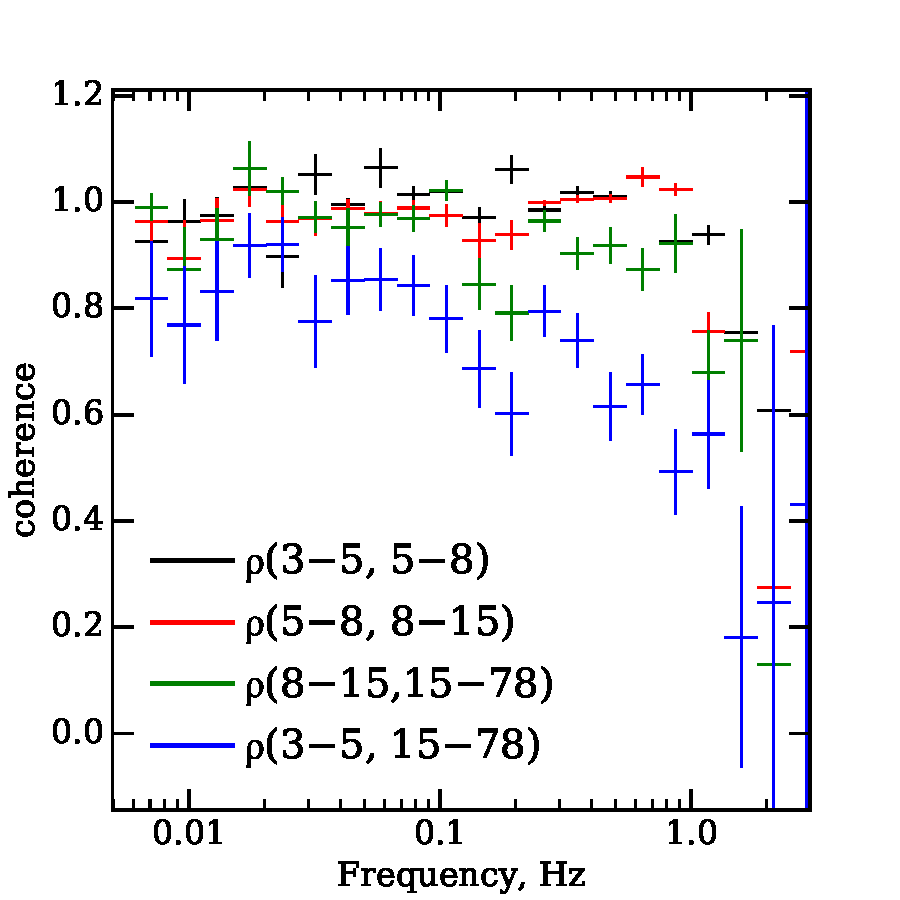
\includegraphics[width=\columnwidth]{coherence_4.pdf}
    \caption{Coherence between different energy bands:  red crosses between 3--5 and 5--8 keV,
     green crosses between 5--8 and 8--15 keV, blue crosses between 8--15 and 15--78 keV, black crosses between 3--5 and 15--78 keV.}
    \label{fig:coherence}
\end{figure}

%It should be noted that while cospectra, used in the denominator of Eq.~\ref{eq:nowak_coh} are not biased due to the Poisson noise, which is not the case for the nominator estimation $|<H(f)^*S(f)>|$. 
%Since in the observation count-rate from \grs\ was relatively low and the Poisson noise contribute significant part in the total rms, we use eq.8 from \citep{1997ApJ...474L..43V} to correct signals intrinsic coherence for polluting Poisson noise component. 
%For the estimation of the Poisson noise component we take square root of the count-rate, thus, we do not consider dead-time effects.  

On Figure~\ref{fig:coherence} presented measured coherence between hard and soft bands on the frequencies up to $\sim1$~Hz. 
We found that coherence in the neighboring energy hands is close to unity, with mean values in 0.01--1~Hz frequency band being $1.0\pm0.05$, however we found that for the 3--5 and 15--78~keV energy bands the coherence is significantly lower, see Fig.~\ref{fig:coherence}. It is on the nearly constant level of $0.85$ in the 0.01--0.3~Hz frequency band and drops down above this frequency.
SInce the loss of the coherence is also observed above 0.3--1.0~Hz frequency for other energy bands, this effect may be connected not with the intrinsic properties of the source, but with the bead-time cross-talk effects which we did not specially consider, except for using light-curves from the different {\it NuSTAR} modules for cross-products.

\subsection{Phase lags}
    
Following \citep{1997ApJ...474L..43V} we estimated phase lag as an angle of mean product of the light curves Fourier harmonics from one energy bands to the conjugated Fourier harmonics of second energy band. 
We can imagine that each light curve from a sample consist of a stochastic noise and coherent signal $S\exp{-i(\alpha(s, h) + U_{h=s}[-\pi, \pi])} + N\exp{-iU[-\pi, \pi]}$, where S and N amplitudes of coherent signals and noise correspondingly and U - uniform distribution, $U_{h=s}$ stands for random phase shift equal for the signals in hard and soft bands, and $\alpha(s, h)$ - phase shift between soft and hard bands.
Therefore the product of the Fourier signals from two bands is $S_{s}S_{h}\exp{-i\alpha(s, h) + (S_{s}*N_{h} + S_{h}*N_{s} + N_{h}*N_{s})\exp{-iU[-\pi, \pi]}}$.
\citep{bachetti17} pointer out that the product of two normally distributed values has probability density function (PDF) of the form of special Bessel function of second kind with zero order. 
It follows that noise components in the Brackets is a sum of three random numbers with PDF = $K_{0}$, with not equal moments, phase of the coherent part is either well defined or distributed around some particular phase shift.
%Result of the product of two Fourier harmonics can be represented as a sum of four complex numbers, amplitude of each is distributed with PDF having a form of modified Bessel function, phases of three of these numbers distributed uniformly, and phase of the last one is distributed nonuniformly with mean equal to real phase shift between two coherent signals.
We can now determine the ``phase axis'' as the axis along the mean complex value of the Sample.
Distribution of the points relative to the ``phase axis'' obviously should be symmetrical, and along it should be assymetric and shifted towards the mean complex value of the sample.
If we now rotate all the obtained complex Fourier harmonics in our sample along this axis $\frac{<P_{\rm hs}^{*}>P_{\rm hs}}{|<P_{\rm hs}>|}$, real part of each value is the projection on the ''phase axis'' and imaginary part is projection on the perpendicular axis. 
We found that the distribution of the projected on the ''phase axis'' values is closely resembles assymetric Laplace distribution and the distribution of the points projected on the perpendicular axis resembles symmetric Laplace distribution. 
Bearing this in mind we estimate mean value for each of the four distributions (positive real, negative real, positive imaginary and negative imaginary) and assess variances of this distribution.
Since we accepted that each of these distribution has a PDF close to exponential we take their variance as a variance of $\chi_2^{\rm 2N}$ distribution, where $N$ - is a number of entities in the each sample. 
After that we accept the error on the phase to be equal $\pi$ if the mean of positive real sample is less than the square root of the sum of the positive and negative real samples variances, otherwise we take it to be equal
\begin{equation}
        \Delta \phi = atan{\left(\frac{\sqrt{v_{i-}^2 + v_{i+}^{2}}}{m_{r+} - m_{r-} - \sqrt{v_{r+}^2 + v_{r-}^2}}\right)}
\end{equation}

    Most of the models of the accretion flow which describe variability and energy spectra formation, suggest the time lag between the signals in different energy bands. 
For example in some models of the energy spectra formation, time lag is naturally arise due to the geometry of the corona and properties of the inverse Comptonization process \citep[see, e.g.][]{kotov01}.
Phase lag is also suggested from the propagating fluctuations model - hard photons are emitted from the inner parts of the accretion flow from the perturbations, which initially were born in the outer parts of the disk were produce soft emission.  

\citep{eijeden17} have found, that the phase lag of XBs, probably depends on the system inclination angle, it also definitely contain information about the characteristic times of the system, and therefore can be proxy to the compact object mass \citep{}. 

Phase lags can be estimated as a product of the mean phase of the set of Fourier spectra and the corresponding frequency:
\begin{equation}
                \tau = \frac{\phi(f)}{2\pi f}\\
\end{equation}
\begin{equation}
        \phi(f) = <arccos{\left(\frac{re(<F_{\rm h}^{*}(f)F_{\rm s}(f)>)}{|F_{\rm h}^{*}(f) F_{\rm s}(f)|}\right)}>
        \label{eq:phase_lag}
\end{equation}
here, $F_h(f)$ and $F_s(f)$ are Fourier functions of the light-curves in the hard and soft bands, $\phi(f)$ is the phase lag. 

%Due to the significant fraction of the Poisson noise in each observation we were not able to obtain phase lag for them.
%We found that phase lag on each frequency is generally conserved along the observation.
%In order to improve significance we compute phase lag for all 13 time series.
Phase lag between 3--5 and 8--15~keV energy bands for frequencies from $10^{-2}$~Hz to 10~Hz is presented in Figure~\ref{fig:phase_lag}.
To measure phase lags we use two approaches, first we estimated with the frequency scaling, as it was described in the previous part, second we estimated phase lag on the raw frequency suggesting that it do not changing with time.
Surprisingly, both pictures appears to be very similar, it should be noted that some observations suggested that the phase lag changes with the QPO frequency \citep{}

It appears that the phase lags is generally positive (hard lag) on the frequencies 0.1--2~Hz, and also can be described with the shifted power law $\propto(f - f_0)^{0.3}$. 
Above 2~Hz significance of the phase lags estimation drops due to the Poisson noise.
In the range 0.03--0.1 Hz there is a week indication on the negative phase lag with the mean value $\approx 0.02\pi$, which corresponds to the time $\approx0.1$~s.



%It Follows from Figure~\ref{fig:phase_lag} that there is soft lag on low frequencies which transforms in to the hard lag on frequencies grater than QPO frequency. 

\begin{figure}
        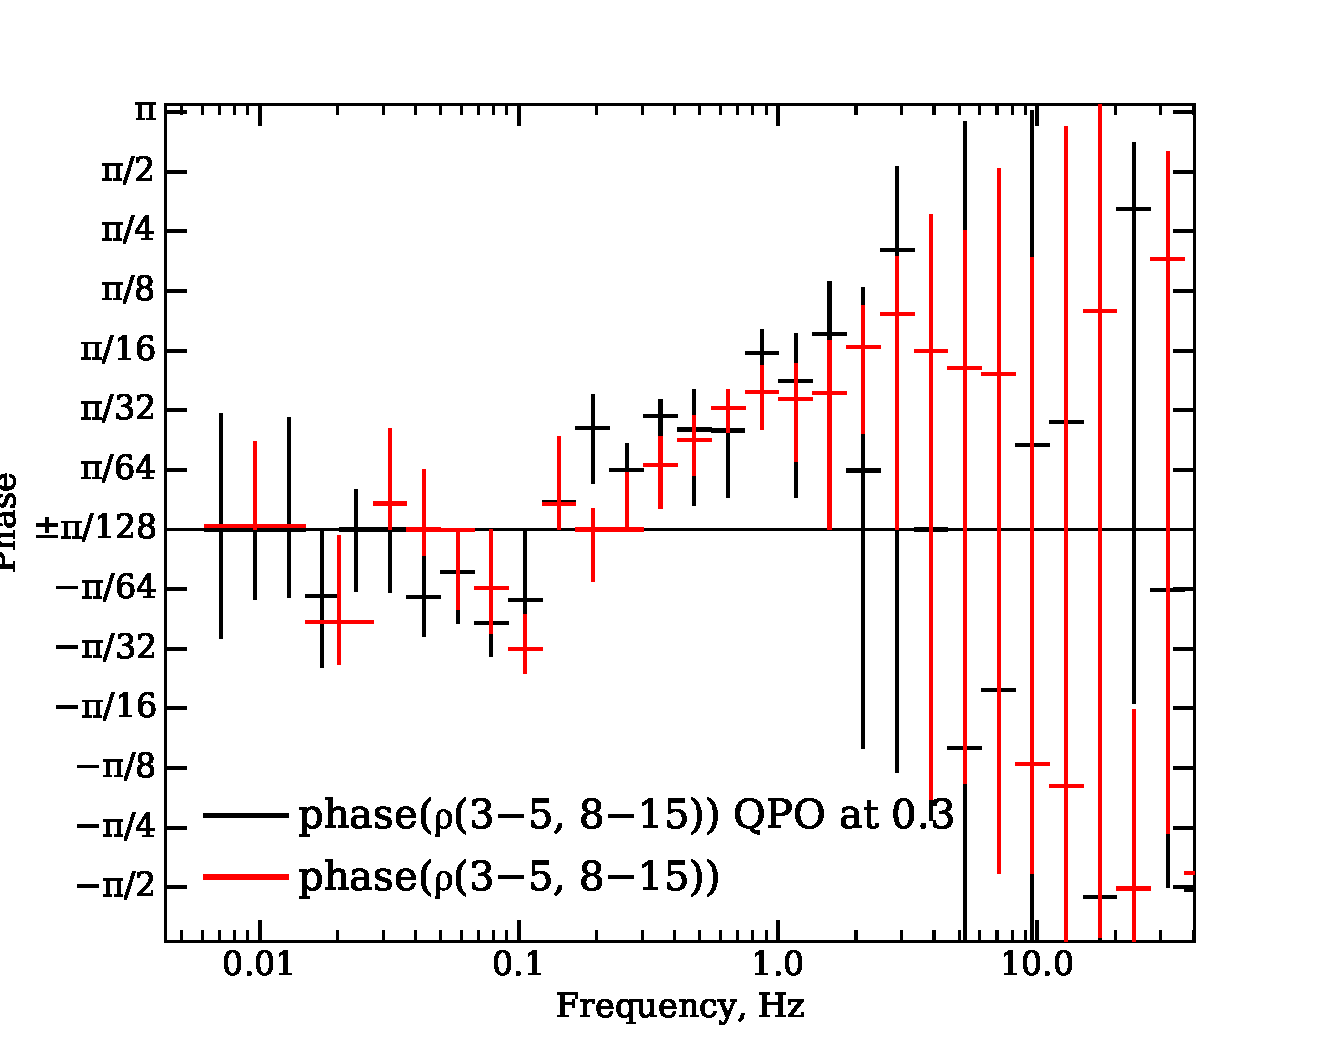
\includegraphics[width=\columnwidth]{phase_lags_traced_and_not.pdf}
        \caption{Phase lag between the hard (3--5~keV) and soft (8--15) energy bands in \grs}
        \label{fig:phase_lag}
\end{figure}

\subsection{\swiftx\, observations}
We performed search for LF QPOs in first dosen of \swiftx observations of the \grs. QPO is clearly detected in observations 3 to 9, with frequency varying from 0.4 Hz (during simultaneous observation with \nustar, see Fig.~\ref{fig:nust_lc}) up to 5 Hz (see Tab.~\ref{tab:xrtqpo}). Due to typically short exposures of \swiftx\, snapshots (about 1 ks) it is hard to classify QPOs as belonging to type C or B, because low-frequency part of power spectra lacks statistics, yet, except for the first detection (segment 03) power spectra were red-noise like, without strong low-frequency components. We calculated $rms$ for each detected QPO - most of them is higher than 10\%, which is not typical for type C QPO \citep{casella05}.

\begin{table}
\noindent
\centering
\caption{QPOs detected in \swiftx\, observations}
\label{tab:xrtqpo}
\centering
\begin{tabular}{|c|c|c|c|}
\hline\hline
Segment & $f_{QPO}$, Hz & $rms$, \% & Type\\
\hline
03  &  0.4  &  14\% & C\\
04  &  2.2 &  11\% & B\\
05  &  1.7  & 13\% & B \\ 
06  &  5.0 &   6\% & B\\
07  &  2.5 &  10\% &  B\\ 
08  &  5.1 &   7\% & B\\
09  &  2.2 &  11\% &  B\\
\hline
\end{tabular}
\end{table}

\section{Discussion}
We had studied the spectra-timing evolution of the \grs\, during its hard-intermediate state.  The frequency of type-C LF QPO show clear correlation with properties of continuum emission. As the QPO frequency increases form 0.3 to 0.7 Hz spectrum became softer: the power law index grows from 1.46 to 1.53 and cut-off energy decreases from 30 to 26 keV. Overall flux increases, too. 
This behaviour was first observed in a number of systems by \citet{dimatteo99} and now it is studied in greater details in many systems \citep[see e.g.][ and many more]{vignarca03,stiele13,seifina14,fuerst16_gx339}. Although the quality of a data prevented us from measuring a movement of the inner disk boundary, from the total broadband spectrum we found that an accretion disk is truncated at radius smaller than 8 $GM/c^{2}$ (90\% confidence limit) which is in agreement with an estimates by \citet{miller15_nust}. This allowed us to check if this combination of inner radius and frequency is consistent with the popular model of QPO generation such as Lense-Thirring precession \citep{ingram09}. Following the calculations of \citet{ingram14} we calulated nodal frequencies (which is though to correspond to QPO fundamental frequency) versus inner radius for two values of black hole mass (10$M_{\odot}$ and 30$M_{\odot}$) and two values of spin - $a=0.1$ and $a=0.998$ (maximally rotating). As it can be seen from Fig.~\ref{fig:qpoconstr} observations are incompatible with expected values for 10$M_{\odot}$ black hole and barely agrees with slowly rotating massive black hole. This results, along with measurements by \cite{fuerst16_gx339}, indicate that there are some tensions between predictions of RPM and truncation radii inferred from spectral fitting.

\begin{figure}
        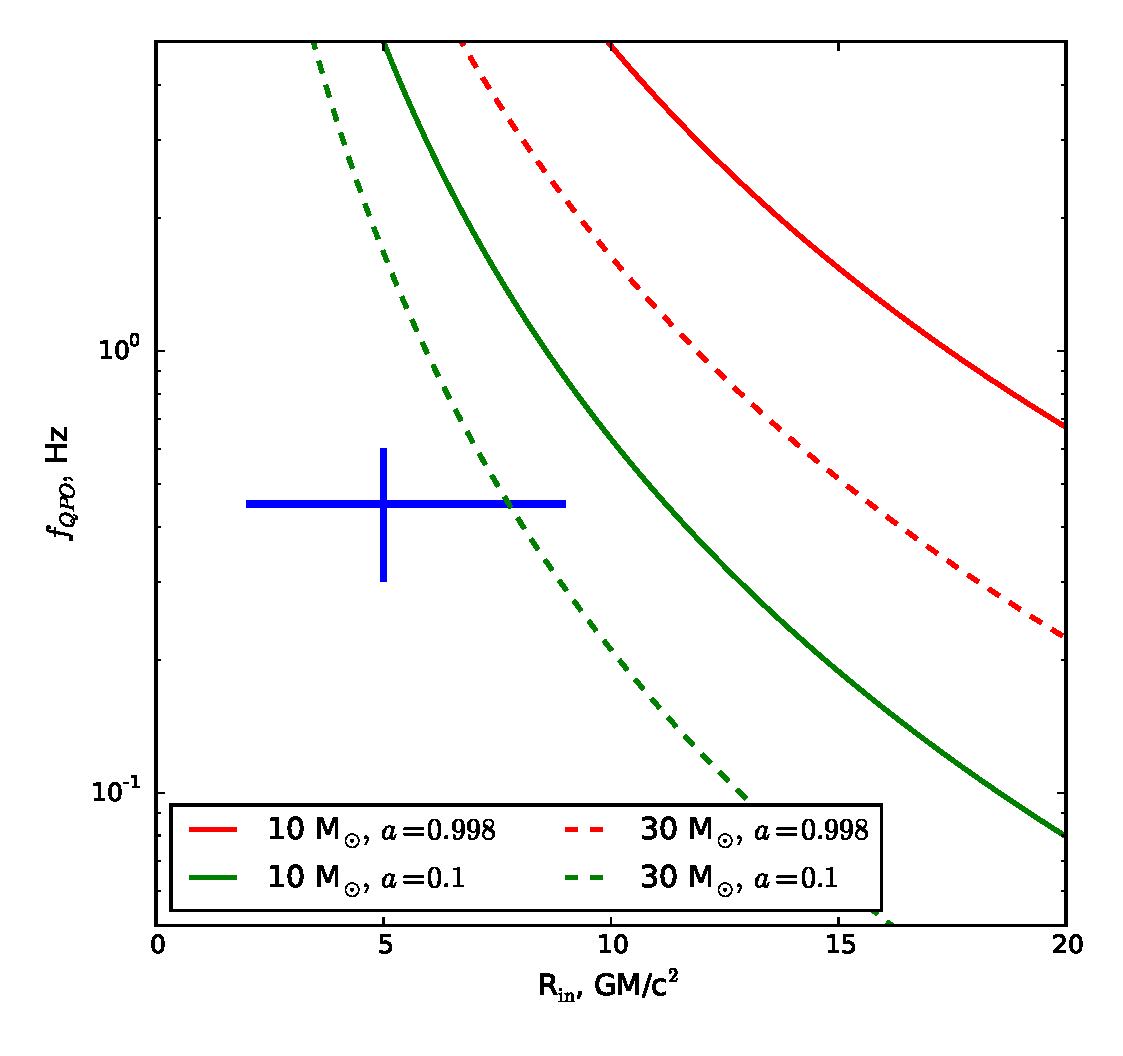
\includegraphics[width=\columnwidth]{qpoconstr_v02.eps}
        \caption{Expected QPO frequency for a black hole of a given mass and spin versus inner disk radius from \cite{ingram14}. Blue point correspond to measured inner disk radius and range of observed QPO frequencies.}
        \label{fig:qpoconstr}
\end{figure}

We carried out extensive study of timing properties of the \grs. Along with broadband noise and fundamental QPO first overtone of QPO is clearly seen. During several intervals from first half of the observation subharmonic was seen too. Break frequency of broadband noise is correlated with QPO frequency following the WK relation \citep{wijnands99}. In all 13 intervals first QPO overtone is more prominent in soft band (3--5 keV), with relation of its amplitude to that of fundamental QPO being 0.4(1) in 3--5 keV band versus 0.2(1) in 10--78 keV.  We also measure velocity of QPO drift and found it to be 7.0\times10^{-6}$~Hz~s$^{-1}$. We searched for similar QPO in \swiftx\, observations of the \grs performed after \nustar\, exposure and found that all other detected QPOs are probably of type B, thus indicating that the type-C QPO reach saturation on frequencies below few Hz. 
Coherence measured between adjacent energy ranges in 0.01-1 Hz was found to be nearly unity, while for distant energy coherence turned out to be lower. Phase lag found to be ....


\section*{Acknowledgments}

%--------------------------------------------------------------------------------
\bibliographystyle{astron}
\bibliography{author_en.bib,coherence.bib}
\bsp	
\label{lastpage}
\end{document}
